
In this thesis, all the simulations are based on the geometry of a skew quadrupole which belongs to the group of high-order corrector magnets designed for the High-Luminosity LHC. The skew quadrupole is developed by LASA laboratories of INFN-Milano. Its geometry is presented in Fig. \ref{fig:Skew_quad_geometry}. Each of the coils of the skew quadrupole (marked in red in the left picture) is fully impregnated and positioned in two mechanical supports (marked in grey). The entire magnet is surrounded by an iron yoke (marked in blue). One coil of a magnet out of four in total is presented in the right picture.

\begin{figure}[H]
    \centering
    \begin{tikzpicture}
    \node at (0,0) {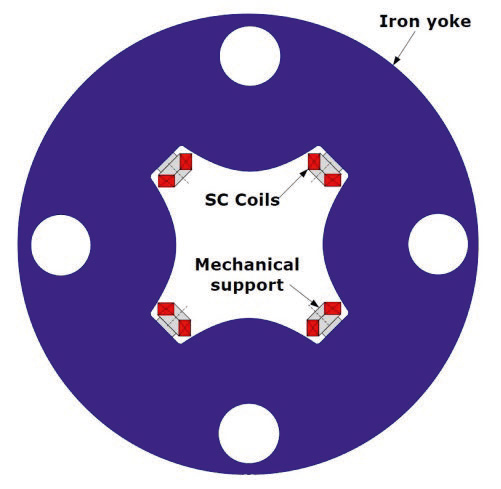
\includegraphics[width=0.3\linewidth]{sections/1D_quench_modelling/figures/geometry/Quadrupole_Cross_Section.png}};
    \node at (5,0) {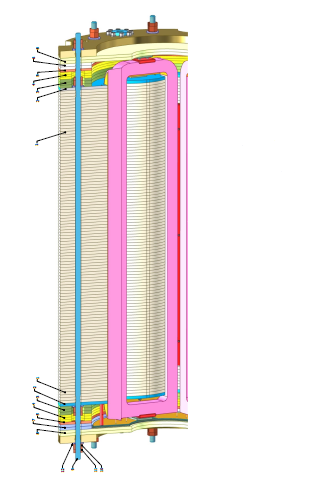
\includegraphics[width=0.225\linewidth]{sections/1D_quench_modelling/figures/geometry/SkewQuad3D.png}};
    \end{tikzpicture}
     \caption{Left: one coil of the skew quadrupole 3D geometry~\cite{marco_prioli_mails}; right: cross-section of the skew quadrupole~\cite[p.~103-105]{hl_lhc_tech_design_report_v01}.}
    \label{fig:Skew_quad_geometry}
\end{figure}

Each coil of the magnet consists of 754 windings which accounts for an 812-metre long cable~\cite{samuele_mariotto_mails}. Every winding is a superconducting strand with a copper stabiliser. It is important to mention that in high-order corrector magnets, the Rutherford cable is not applied. The 1D geometry is based on geometrical parameters of a single strand of a skew quadrupole whose simulations are further described in the next section. As presented in Fig.~\ref{fig: 1d_strand_geometry}, the coil consists of a strand with a circular cross-section (in yellow). The composite strand is made of Nb-Ti with copper as a stabiliser. The composite is fully insulated with an S2-glass material (in red). Then, the strand with the insulation layer is immersed in D10 epoxy resin (in blue)~\cite[p.~103-105]{hl_lhc_tech_design_report_v01}. The one-dimensional coordinate system $\bar x$ in Fig.~\ref{fig: 1d_strand_geometry} represents the longitudinal direction of the strand.

\begin{figure}[H]
    \centering
    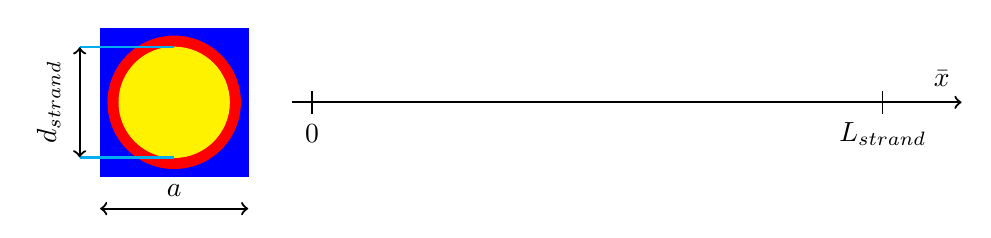
\begin{tikzpicture}[scale = 1]
        \filldraw[blue] (-0.941,-0.941) rectangle (0.941,0.941);
        \filldraw[red] (0,0) circle (0.7+0.07*2);
        \filldraw[yellow] (0,0) circle (0.7);
        \draw[thick, cyan] (-0.8*1.5,0.7) -- (0,0.7);
        \draw[thick, cyan] (-0.8*1.5,-0.7) -- (0,-0.7);
        \draw[black, thick, <->] (-0.75*1.6,0.7) -- (-0.75*1.6,-0.7);
        \node[scale = 1, rotate=90] at (-1.1*1.45, 0) {$d_\text{strand}$};
        \draw[thick,<->] (-0.941,-0.9*1.5) -- (0.941,-0.9*1.5);
        \node[scale = 1] at (0, -0.7*1.6) {$a$};
        \draw[thick,->] (1.5,0) -- (10.0,0);
        \draw[thin] (1.75,-0.15) -- (1.75,0.15);
        \draw[thin] (9,-0.15) -- (9,0.15);
        
        \node[scale = 1] at (9.75, 0.3) {$\bar x$};
        \node[scale = 1] at (9, -0.4) {$L_\text{strand}$};
        \node[scale = 1] at (1.75, -0.4) {0};
        
    \end{tikzpicture}
    \caption{1D strand geometry.}
    \label{fig: 1d_strand_geometry}
\end{figure}

The parameters of the skew quadrupole are presented in Table \ref{table:skew_quad_params_table_basic}. None of the presented parameters change in the remainder of the thesis. The last two: $(i)$ residual resistivity ratio, RRR, $(ii)$ copper-to-superconductor ratio, $r_\text{Cu/Nb-Ti}$ are obtained from the measurements of the prototype magnet performed at INFN~\cite{marco_prioli_mails}.

\begin{table}[H]
    \caption{Geometrical parameters of the skew quadrupole \cite{marco_prioli_mails, hl_lhc_tech_design_report_v01}.} 
    \vspace{-1.em} 
    \fontsize{10}{10}
    \selectfont 
    \renewcommand{\arraystretch}{1.5}
    \begin{center}
    \begin{tabular}{ ccc }  
    \hline
    parameter & value & unit \\
    \hline
    strand diameter, $d_\text{strand}$ & 0.7 & [mm] \\
    strand side, $a$ & 0.941 & [mm] \\
    $r_\text{Cu/Nb-Ti}$ & 2.2 & [-] \\
    RRR & 193 & [-] \\  
    \hline 
    \end{tabular}
    \end{center}  
     \label{table:skew_quad_params_table_basic} 
 \end{table}
